\documentclass{beamer}
\mode<presentation>
{
  \usetheme{Madrid}
  \usecolortheme{beaver}
  \usefonttheme{serif}
  \setbeamertemplate{navigation symbols}{}
  \setbeamertemplate{caption}[numbered]
  \setbeamercolor{theorem}{fg=red}
  \usepackage{amssymb}
  \usepackage{mathtools}
  \usepackage[english]{babel}
  \usepackage[utf8x]{inputenc}
  \usepackage{xcolor}
  \usepackage{ifthen}

  \usepackage{listings}
  \usepackage{wasysym}
  \usepackage{tikz}
  \usetikzlibrary{tikzmark}
  \lstset{
      language=[LaTeX]TeX,
      breaklines=true,
      basicstyle=\tt\scriptsize,
      keywordstyle=\color{magenta},
      stringstyle=\color{black},
      identifierstyle=\color{magenta},
  }
}

\title[]{Introduction to Reinforcement Learning}
\subtitle{\url{https://github.com/racousin/rl_introduction}}
\author{Raphael Cousin}
\date{March 4, 2024}

\AtBeginSection[]
{
  \begin{frame}<beamer>
    \frametitle{Agenda}
    \tableofcontents[currentsection,currentsubsection]
  \end{frame}
}

\newcommand{\arrowright}{\tikz \draw[->, thick] (0,0) -- (0.3,0);}
\newcommand{\arrowleft}{\tikz \draw[<-, thick] (0,0) -- (0.3,0);}
\newcommand{\arrowup}{\tikz \draw[->, thick] (0,0) -- (0,0.3);}

\begin{document}

\begin{frame}
  \titlepage
\end{frame}





\begin{frame}{Course Objectives}
    \begin{itemize}
\item{The keys to go by yourself in RL}

\item{Practice coding}

\item{General culture}
    \end{itemize}
What do you already know about RL?
\end{frame}

\begin{frame}{Why reinforcement learning?}
        \begin{figure}
        \centering
        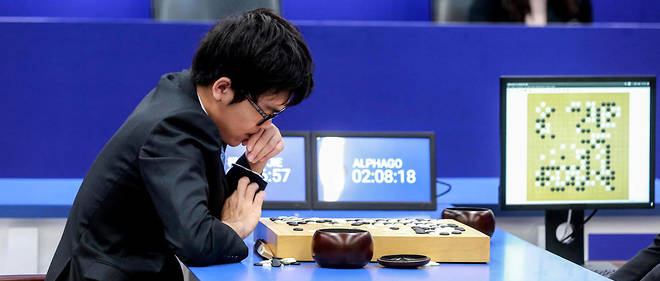
\includegraphics[height=4cm]{alphago.jpg}
        \caption{In 2017, AlphaGo defeated Ke Jie, the world's top-ranked Go player.}
    \end{figure}
\end{frame}

\begin{frame}{RL vs. Other Machine Learning Paradigms}
    \begin{itemize}
        \item Supervised Learning: Learning from labeled data to predict outcomes.
        \item Unsupervised Learning: Finding patterns in data without explicit labels.
        \item Reinforcement Learning: Learning decision-making by interacting with an environment to achieve goals.
    \end{itemize}
    In contrast to the other two, RL is focused on learning from the consequences of actions.
\end{frame}

\begin{frame}{The RL Framework}
    \begin{itemize}
        \item Absence of explicit "correct" actions.
        \item Learning is guided by rewards that represent the objectives.
    \end{itemize}
    \begin{figure}
        \centering
        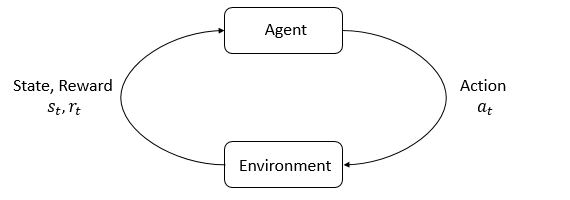
\includegraphics[height=4cm]{rl.png}
        \caption{The agent-environment interaction in RL.}
    \end{figure}
\end{frame}

\begin{frame}{Applications of RL}
    RL has been successfully applied in various fields, including:
    \begin{itemize}
        \item Autonomous vehicles/Robotics
        \item Control systems
        \item Chat bots policy
        \item Marketing/Trading strategies
        \item Game playing and beyond
    \end{itemize}
    \begin{figure}
        \centering
        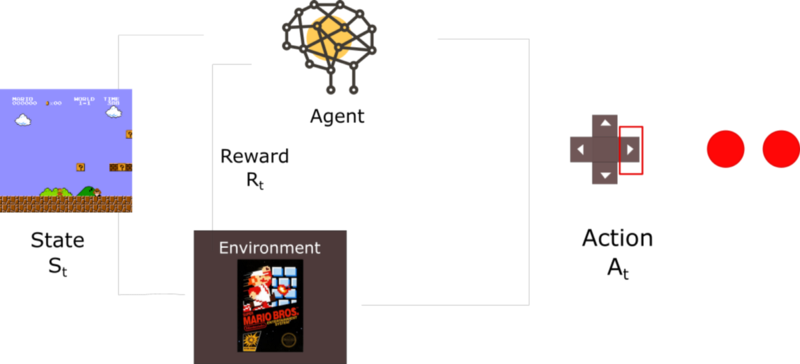
\includegraphics[height=4cm]{game.png}
        \caption{RL in video games.}
    \end{figure}
\end{frame}


\begin{frame}{Course Outline}
    \begin{itemize}
        \item I) Understanding Markov Decision Processes (MDPs)
        \item II) Exploring Model-Free Reinforcement Learning
        \item III) Diving into Deep Reinforcement Learning
    \end{itemize}
    We'll start with the basics and gradually move to more complex concepts.
\end{frame}


\begin{frame} {I) Understanding Markov Decision Processes}
    \begin{figure}
        \centering
        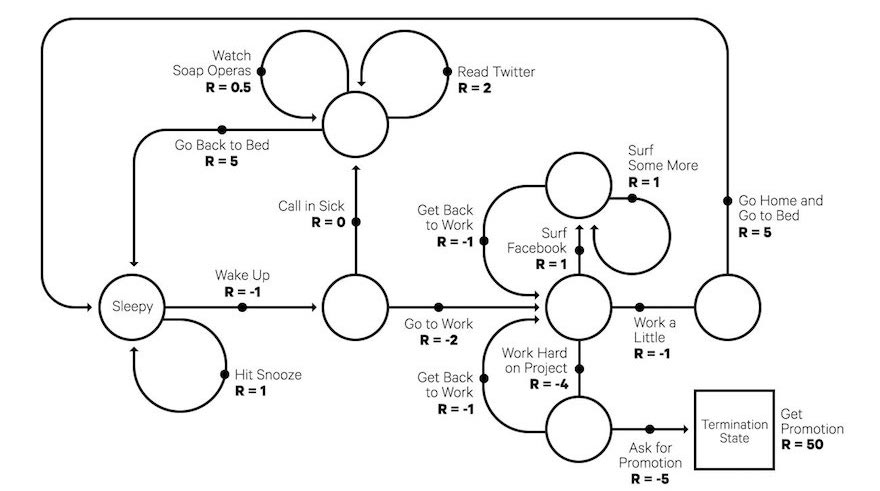
\includegraphics[height=6.4cm]{mdp.jpg}
        \caption{Illustrative example of an MDP, showcasing state transitions, actions, and rewards.}
    \end{figure}
\end{frame}

\begin{frame}{First Glossary of MDPs}
    \begin{itemize}
        \item State Space ($S$)
        \item Action Space ($A$)
        \item Transition Model ($P$)
        \item Reward function ($R$)
        \item Policy ($\pi$)
        \item Trajectory ($\tau$)
        \item Return ($G$)
    \end{itemize}
\end{frame}

\begin{frame}{Simple Grid World Problem}
    \begin{center}
        \normalsize Our environment is a 4x4 grid where an agent aims to reach a goal.
    \end{center}
    \begin{figure}
        \centering
        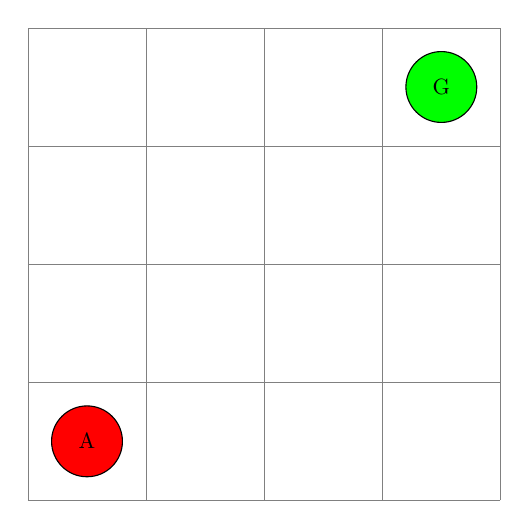
\begin{tikzpicture}[scale=1.5, every node/.style={scale=0.8}]
            \draw[step=1cm,gray,very thin] (0,0) grid (4,4);
            \draw[fill=green] (3.5,3.5) circle (0.3cm); % Goal
            \draw[fill=red] (0.5,0.5) circle (0.3cm); % Agent
            \node at (3.5, 3.5) {G};
            \node at (0.5, 0.5) {A};
            \foreach \x in {0,...,3}
                \foreach \y in {0,...,3}
                    \node[draw=none] at (\x+0.5,\y+0.5) {}; % Centers
        \end{tikzpicture}
        \caption{A: Agent, G: Goal}
    \end{figure}
\end{frame}



\begin{frame}{State Space ($S$)}
    \begin{center}
        \large 16 discrete states.\\
        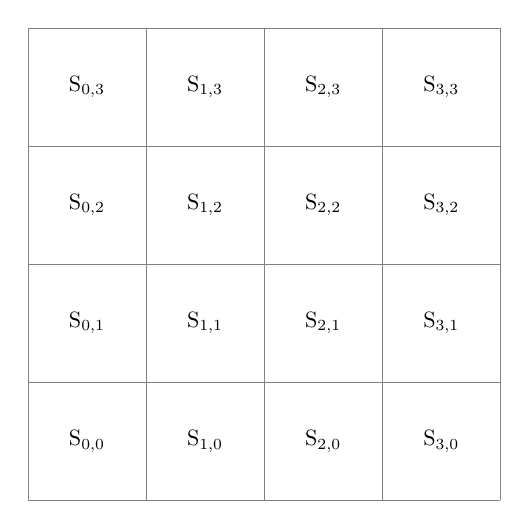
\begin{tikzpicture}[scale=1.5, every node/.style={scale=0.8}]
            \draw[step=1cm,gray,very thin] (0,0) grid (4,4);
            \foreach \x in {0,...,3}
                \foreach \y in {0,...,3}
                    \node[draw=none] at (\x+0.5,\y+0.5) {S\textsubscript{\x,\y}};
        \end{tikzpicture}
    \end{center}
\end{frame}




\begin{frame}{Action Space ($A$)}
    \begin{center}
        \large 4 discrete actions (Up, Down, Left, Right).
        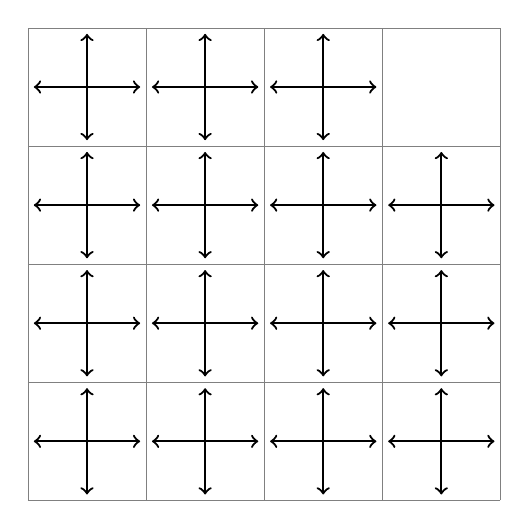
\begin{tikzpicture}[scale=1.5, every node/.style={scale=0.8}]
            \draw[step=1cm,gray,very thin] (0,0) grid (4,4);
            % Loop over each cell to draw arrows
            \foreach \x in {0,...,3}
                \foreach \y in {0,...,3}
                {
                \ifthenelse{\NOT \x = 3 \OR \NOT \y = 3}{  
                    % Up arrow
                    \draw[->, thick] (\x+0.5,\y+0.5) -- (\x+0.5,\y+0.95);
                    % Down arrow
                    \draw[->, thick] (\x+0.5,\y+0.5) -- (\x+0.5,\y+0.05);
                    % Left arrow
                    \draw[->, thick] (\x+0.5,\y+0.5) -- (\x+0.05,\y+0.5);
                    % Right arrow
                    \draw[->, thick] (\x+0.5,\y+0.5) -- (\x+0.95,\y+0.5);
                    }
                }
        \end{tikzpicture}
    \end{center}
\end{frame}





\begin{frame}{Transition Model: $P_{ss'}^a = \mathbb{P} [S_{t+1} = s' \vert S_t = s, A_t = a]$}
    \begin{center}
        \large Deterministic environment.\\
        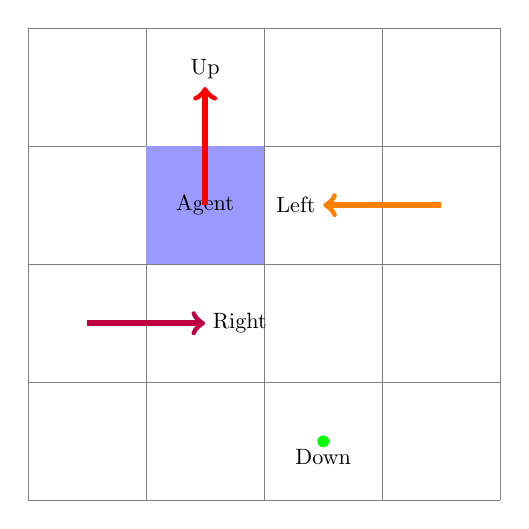
\begin{tikzpicture}[scale=1.5, every node/.style={scale=0.8}]
            \draw[step=1cm,gray,very thin] (0,0) grid (4,4);
            
            % Example current position
            \fill[blue!40!white] (1,2) rectangle (2,3);
            \node at (1.5,2.5) {Agent};
            
            % Example transition
            % Up arrow
            \draw[->, line width=2pt, red] (1.5,2.5) -- (1.5,3.5);
            \node[above] at (1.5,3.5) {Up};
            
            % Down arrow
            \draw[fill=green,draw=none] (2.5,0.5) circle (0.05cm); % Small
            \node[below] at (2.5,0.5) {Down};
            
            % Left arrow
            \draw[->, line width=2pt, orange] (3.5,2.5) -- (2.5,2.5);
            \node[left] at (2.5,2.5) {Left};
            
            % Right arrow
            \draw[->, line width=2pt, purple] (0.5,1.5) -- (1.5,1.5);
            \node[right] at (1.5,1.5) {Right};
            
        \end{tikzpicture}
    \end{center}
\end{frame}

\begin{frame}{Transition Model: $P_{ss'}^a = \mathbb{P} [S_{t+1} = s' \vert S_t = s, A_t = a]$}
    \begin{center}
        \large Stochastic environment.\\
        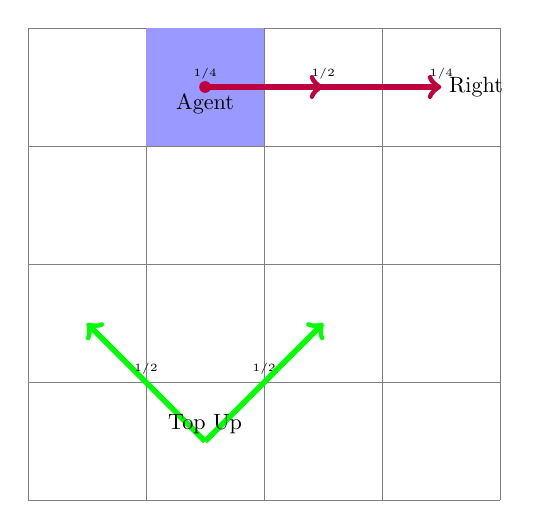
\begin{tikzpicture}[scale=1.5, every node/.style={scale=0.8}]
            \draw[step=1cm,gray,very thin] (0,0) grid (4,4);
            
            % Agent in cell (2,2) with possible moves
            \fill[blue!40!white] (1,3) rectangle (2,4);
            \node[above] at (1.5,3.5) {\tiny $1/4$};
            \node[below] at (1.5,3.5) {Agent};
            \draw[fill=purple,draw=none] (1.5,3.5) circle (0.05cm);
            
            
            % Move to cell (3,2)
            \draw[->, line width=2pt, purple] (1.5,3.5) -- (2.5,3.5);
            \node[above] at (2.5,3.5) {\tiny $1/2$};
            
            % Move to cell (4,2)
            \draw[->, line width=2pt, purple] (1.5,3.5) -- (3.5,3.5);
            \node[above] at (3.5,3.5) {\tiny $1/4$};
            \node[right] at (3.5,3.5) {Right};
            
            \draw[->, line width=2pt, green] (1.5,0.5) -- (0.5,1.5);
            \node[above] at (2,1) {\tiny $1/2$};
            \draw[->, line width=2pt, green] (1.5,0.5) -- (2.5,1.5);
            \node[above] at (1,1) {\tiny $1/2$};
            \node[above] at (1.5,0.5) {Top Up};
        \end{tikzpicture}
    \end{center}
\end{frame}




\begin{frame}{Reward function: $r = R(s, a) = r(s')$}
    \begin{center}
        \large Simple goal reward.\\
        % \normalsize +1 for reaching G, 0 otherwise.
        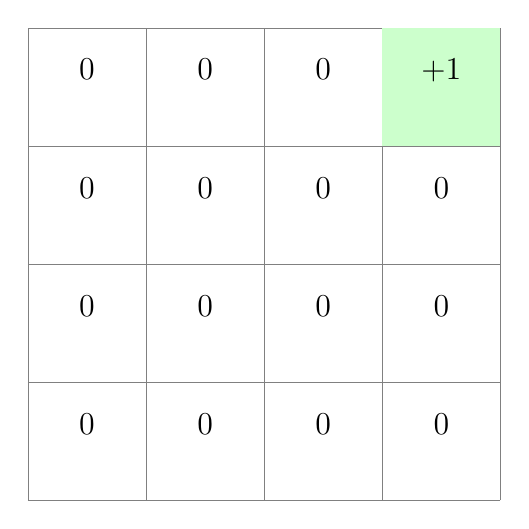
\begin{tikzpicture}[scale=1.5, every node/.style={scale=0.8}]
            \draw[step=1cm,gray,very thin] (0,0) grid (4,4);
            
            % Goal cell with reward
            \fill[green!20] (3,3) rectangle (4,4); % Highlight goal cell
            % \node at (3.5,3.5) {G};
            \node[below] at (3.5,3.8) {\Large +1};
            
            % Other cells with default reward
            \foreach \x in {0,...,3}
                \foreach \y in {0,...,3}
                {
                    \ifthenelse{\NOT \x = 3 \OR \NOT \y = 3}
                    {\node[below] at (\x+0.5,\y+0.8) {\Large 0};}{}
                }
        \end{tikzpicture}
    \end{center}
\end{frame}

\begin{frame}{Reward function: $r = R(s, a) = r(s')$}
    \begin{center}
        \large Other example of environment reward function.\\
        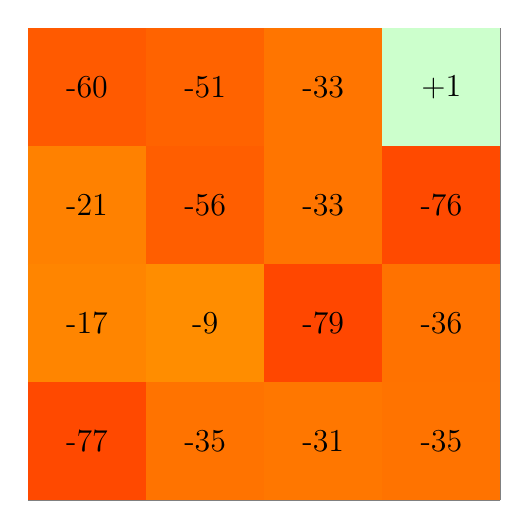
\begin{tikzpicture}[scale=1.5, every node/.style={scale=0.8}]
            \draw[step=1cm,gray,very thin] (0,0) grid (4,4);

            % Goal cell with positive reward
            \fill[green!20] (3,3) rectangle (4,4);
            \node at (3.5,3.5) {\Large +1};

            % Other cells with negative rewards
            \foreach \x in {0,...,3}
                \foreach \y in {0,...,3} {
                \ifthenelse{\NOT \x = 3 \OR \NOT \y = 3}{                    % Calculate a random negative reward for each cell
                    \pgfmathsetmacro{\reward}{int(random(-90,-1))}
                    % Calculate color based on reward
                    \pgfmathsetmacro{\colorpercentage}{int(150 + \reward)} % -10 will correspond to 0, -1 to 90
                    \definecolor{currentcolor}{RGB}{255,\colorpercentage,0}
                    \fill[currentcolor] (\x,\y) rectangle (\x+1,\y+1);
                    \node at (\x+0.5,\y+0.5) {\Large \reward};
                }}

        \end{tikzpicture}
    \end{center}
\end{frame}



\begin{frame}{Policy: ($\pi: S \rightarrow A $)}
    \begin{center}
        \Large Agent action in a state defined by its policy deterministic/stochastic\\
        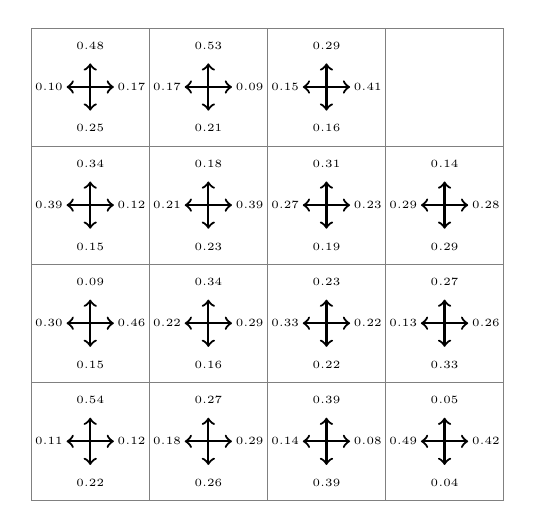
\begin{tikzpicture}[scale=1.5, every node/.style={scale=0.8}]
            \draw[step=1cm,gray,very thin] (0,0) grid (4,4);
            % Loop over each cell to draw arrows with random probabilities
            \foreach \x in {0,...,3}
                \foreach \y in {0,...,3}
                {
                                    % Generate four random numbers
                    \pgfmathsetmacro{\probup}{rnd}
                    \pgfmathsetmacro{\probdown}{rnd}
                    \pgfmathsetmacro{\probleft}{rnd}
                    \pgfmathsetmacro{\probright}{rnd}
                    % Calculate their sum
                    \pgfmathsetmacro{\sumprobs}{\probup + \probdown + \probleft + \probright}
                    % Normalize to sum up to 1
                    \pgfmathsetmacro{\probupnorm}{\probup / \sumprobs}
                    \pgfmathsetmacro{\probdownnorm}{\probdown / \sumprobs}
                    \pgfmathsetmacro{\probleftnorm}{\probleft / \sumprobs}
                    \pgfmathsetmacro{\probrightnorm}{\probright / \sumprobs}
                    % Draw arrows for each direction
                    % Up arrow
                    \ifthenelse{\NOT \x = 3 \OR \NOT \y = 3}{  
                    \draw[->, thick] (\x+0.5,\y+0.5) -- (\x+0.5,\y+0.7);
                    \node at (\x+0.5,\y+0.85) {\tiny \pgfmathprintnumber[fixed, fixed zerofill, precision=2]{\probupnorm}};
                    % Down arrow
                    \draw[->, thick] (\x+0.5,\y+0.5) -- (\x+0.5,\y+0.3);
                    \node at (\x+0.5,\y+0.15) {\tiny \pgfmathprintnumber[fixed, fixed zerofill, precision=2]{\probdownnorm}};
                    % Left arrow
                    \draw[->, thick] (\x+0.5,\y+0.5) -- (\x+0.3,\y+0.5);
                    \node at (\x+0.15,\y+0.5) {\tiny \pgfmathprintnumber[fixed, fixed zerofill, precision=2]{\probleftnorm}};
                    % Right arrow
                    \draw[->, thick] (\x+0.5,\y+0.5) -- (\x+0.7,\y+0.5);
                    \node at (\x+0.85,\y+0.5) {\tiny \pgfmathprintnumber[fixed, fixed zerofill, precision=2]{\probrightnorm}};}
                    }
        \end{tikzpicture}
    \end{center}
\end{frame}



\begin{frame}{Trajectory: $\tau_{\pi} = (s_0, a_0, s_1, a_1, ...)$}
    \begin{center}
    \makebox[\textwidth][c]{\small ($s_{0,0}$, \arrowright, 0, $s_{1,0}$, \arrowright, 0, $s_{2,0}$, \arrowup, 0, $s_{2,1}$, \arrowup, 0, $s_{2,2}$, \arrowleft, 0, $s_{1,2}$, \arrowup, 0, $s_{1,3}$, \arrowright, 0, $s_{2,3}$, \arrowright, 1)}
        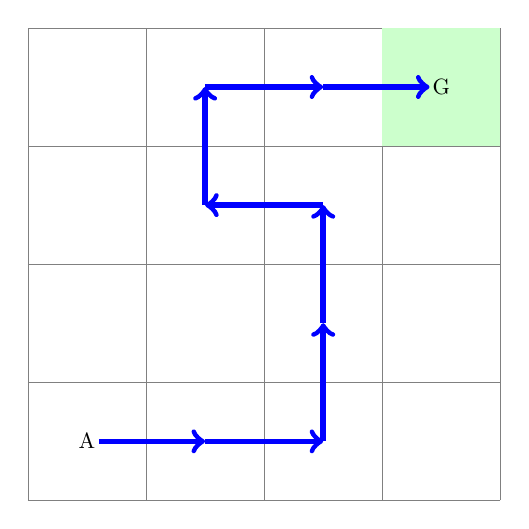
\begin{tikzpicture}[scale=1.5, every node/.style={scale=0.8}]
            \draw[step=1cm,gray,very thin] (0,0) grid (4,4);
            % Goal
            \fill[green!20] (3,3) rectangle (4,4);
            \node at (3.5,3.5) {G};
            % Agent path
            \draw[->, line width=2pt, blue] (0.6,0.5) -- (1.5,0.5);
            \draw[->, line width=2pt, blue] (1.5,0.5) -- (2.5,0.5);
            \draw[->, line width=2pt, blue] (2.5,0.5) -- (2.5,1.5);
            \draw[->, line width=2pt, blue] (2.5,1.5) -- (2.5,2.5);
            \draw[->, line width=2pt, blue] (2.5,2.5) -- (1.5,2.5);
            \draw[->, line width=2pt, blue] (1.5,2.5) -- (1.5,3.5);
            \draw[->, line width=2pt, blue] (1.5,3.5) -- (2.5,3.5);
            \draw[->, line width=2pt, blue] (2.5,3.5) -- (3.4,3.5);
            \node at (0.5,0.5) {A};
        \end{tikzpicture}

    \end{center}
\end{frame}





\begin{frame}{Return: $G_t=\sum_{k=1}^T \gamma^k r_{t+k}$}
    \begin{columns}
        \column{0.5\textwidth}
        \centering
        \textbf{Cumulative rewards}\\
        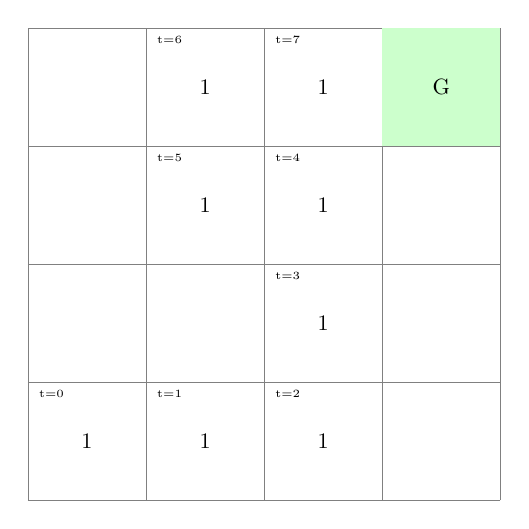
\begin{tikzpicture}[scale=1.5, every node/.style={scale=0.8}]
            \draw[step=1cm,gray,very thin] (0,0) grid (4,4);
            % Goal
            \fill[green!20] (3,3) rectangle (4,4);
            \node at (3.5,3.5) {G};
            % Agent path
            \node at  (0.5,0.5) {1};
            \node at  (0.2,0.9) {\tiny t=0};
            \node at (1.5,0.5) {1};
                        \node at  (1.2,0.9) {\tiny t=1};
            \node at  (2.5,0.5) {1};
                        \node at  (2.2,0.9) {\tiny t=2};
            \node at  (2.5,1.5) {1};
                        \node at  (2.2,1.9) {\tiny t=3};
            \node at  (2.5,2.5) {1};
                        \node at  (2.2,2.9) {\tiny t=4};
            \node at  (1.5,2.5) {1};
                        \node at  (1.2,2.9) {\tiny t=5};
            \node at  (1.5,3.5) {1};
                        \node at  (1.2,3.9) {\tiny t=6};
            \node at  (2.5,3.5) {1};
                        \node at  (2.2,3.9) {\tiny t=7};
        \end{tikzpicture}
        
        \column{0.5\textwidth}
        \centering
        \textbf{Discounted rewards ($0.95$)}\\
        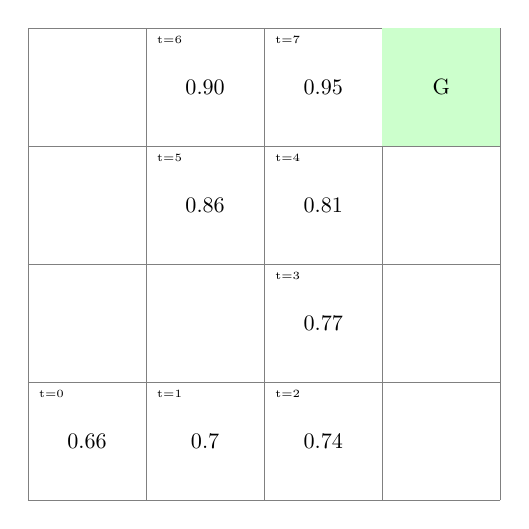
\begin{tikzpicture}[scale=1.5, every node/.style={scale=0.8}]
            \draw[step=1cm,gray,very thin] (0,0) grid (4,4);
            % Goal
            \fill[green!20] (3,3) rectangle (4,4);
            \node at (3.5,3.5) {G};
            % Agent path
            \node at  (0.5,0.5) {0.66};
            \node at  (0.2,0.9) {\tiny t=0};
            \node at (1.5,0.5) {0.7};
            \node at  (1.2,0.9) {\tiny t=1};
            \node at  (2.5,0.5) {0.74};
            \node at  (2.2,0.9) {\tiny t=2};
            \node at  (2.5,1.5) {0.77};
            \node at  (2.2,1.9) {\tiny t=3};
            \node at  (2.5,2.5) {0.81};
            \node at  (2.2,2.9) {\tiny t=4};
            \node at  (1.5,2.5) {0.86};
            \node at  (1.2,2.9) {\tiny t=5};
            \node at  (1.5,3.5) {0.90};
            \node at  (1.2,3.9) {\tiny t=6};
            \node at  (2.5,3.5) {0.95};
            \node at  (2.2,3.9) {\tiny t=7};
        \end{tikzpicture}
    \end{columns}
\end{frame}





\begin{frame}{Objective: Find best Policy $\pi^* = \arg \max_{\pi} E_{\tau\sim \pi}[{G(\tau)}]}
    \begin{center}
    \normalsize Optimal policy in the grid world environment.
        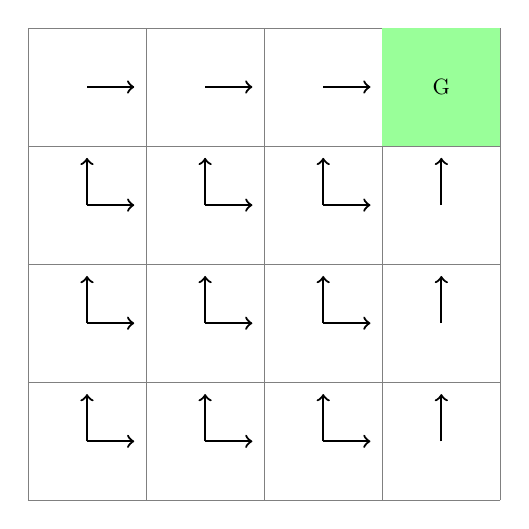
\begin{tikzpicture}[scale=1.5, every node/.style={scale=0.8}]
            \draw[step=1cm,gray,very thin] (0,0) grid (4,4);
            % Goal
            \fill[green!40!white] (3,3) rectangle (4,4);
            \node at (3.5,3.5) {G};
            
            % Arrows pointing towards the goal "G"
            % Right arrows
            \foreach \y in {0,...,3}
                \foreach \x in {0,...,2}
                {
                    \draw[->, thick] (\x+0.5,\y+0.5) -- (\x+0.9,\y+0.5);
                }
            % Up arrows
            \foreach \x in {0,...,3}
                \foreach \y in {0,...,2}
                {
                    \draw[->, thick] (\x+0.5,\y+0.5) -- (\x+0.5,\y+0.9);
                }
                
            
        \end{tikzpicture}
    \end{center}
\end{frame}


\begin{frame}[plain,c]
\begin{center}
    \Huge Let's Code: Environment and Agent Interaction
\end{center}
\end{frame}

\begin{frame}{Second Glossary of MDPs}
    \begin{itemize}
        \item Value Function ($V$)
        \item Action Value Function ($Q$)
        \item Bellman Equations
        \item Dynamic Programming
    \end{itemize}
\end{frame}


\begin{frame}{Value Function: $    V^{\pi}(s) =  E_{\tau \sim \pi}[{G_t\left| S_t = s\right.}]   $}
    \begin{center}
        \Large Expected Return for State following $\pi$
        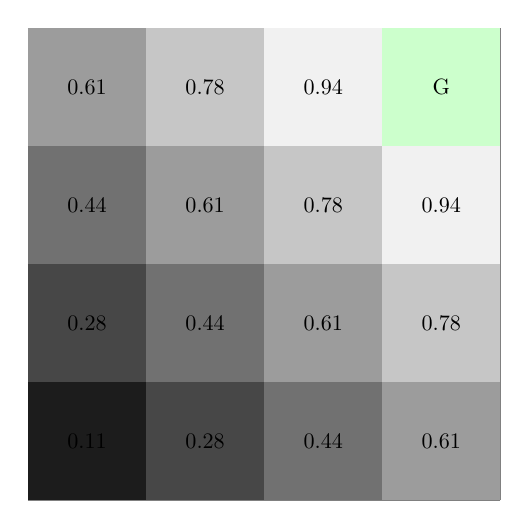
\begin{tikzpicture}[scale=1.5, every node/.style={scale=0.8}]
            \draw[step=1cm,gray,very thin] (0,0) grid (4,4);
            % Goal
            \fill[green!20] (3,3) rectangle (4,4);
            \node at (3.5,3.5) {G};

            % Define a simple value function
            % Let's assume the further you are from the goal (3,3), the lower the value
            \foreach \x in {0,...,3}
                \foreach \y in {0,...,3}
                {
                \ifthenelse{\NOT \x = 3 \OR \NOT \y = 3}{
                    % Calculate a value based on distance from the goal
                    \pgfmathsetmacro{\distance}{abs(\x-3) + abs(\y-3)}
                    \pgfmathsetmacro{\value}{1.11 - (\distance/6)}
                    \definecolor{CurrentValueColor}{rgb}{\value, \value, \value}
                    \fill[CurrentValueColor] (\x,\y) rectangle (\x+1,\y+1);
                    \node at (\x+0.5,\y+0.5) {\pgfmathprintnumber[fixed, fixed zerofill, precision=2]{\value}};
                }}
        \end{tikzpicture}
    \end{center}
\end{frame}

\begin{frame}{Action Value Function:  $Q^{\pi}(s,a) = E_{\tau \sim \pi}[{G_t\left| S_t = s, A_t = a\right.}]$}
    \begin{center}
        \Large Expected Return for State-Action following $\pi$
        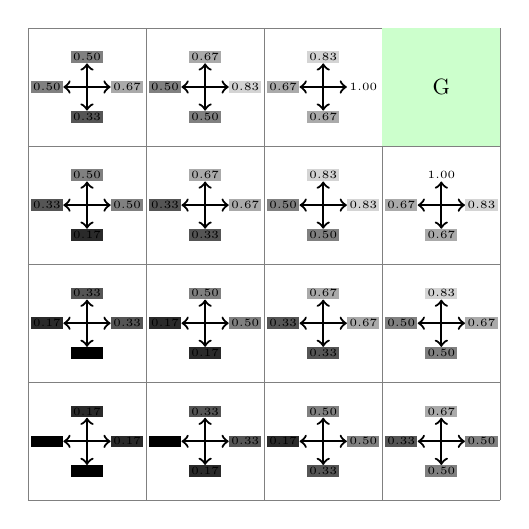
\begin{tikzpicture}[scale=1.5, every node/.style={scale=0.8}]
            \draw[step=1cm,gray,very thin] (0,0) grid (4,4);
            % Goal
            \fill[green!20] (3,3) rectangle (4,4);
            \node at (3.5,3.5) {G};

            % Loop over each cell to display Q-values for each action
            \foreach \x in {0,...,3}
                \foreach \y in {0,...,3}
                {
                
                    % Calculate Q-values based on Manhattan distance to the goal from the current cell
                    \pgfmathtruncatemacro{\UpY}{min(3,\y+1)}
                    \pgfmathtruncatemacro{\DownY}{max(0,\y-1)}
                    \pgfmathtruncatemacro{\LeftX}{max(0,\x-1)}
                    \pgfmathtruncatemacro{\RightX}{min(3,\x+1)}

                    % Calculate Manhattan distances for each action
                    \pgfmathsetmacro{\QupD}{abs(\x-3) + abs(\UpY-3)}
                    \pgfmathsetmacro{\QdownD}{abs(\x-3) + abs(\DownY-3)}
                    \pgfmathsetmacro{\QleftD}{abs(\LeftX-3) + abs(\y-3)}
                    \pgfmathsetmacro{\QrightD}{abs(\RightX-3) + abs(\y-3)}

                    \pgfmathsetmacro{\QupValue}{1 - (\QupD/6)}
                    \pgfmathsetmacro{\QdownValue}{1 - (\QdownD/6)}
                    \pgfmathsetmacro{\QleftValue}{1 - (\QleftD/6)}
                    \pgfmathsetmacro{\QrightValue}{1 - (\QrightD/6)}
                    
                    \definecolor{ColorUp}{rgb}{\QupValue, \QupValue, \QupValue}
                    \definecolor{ColorDown}{rgb}{\QdownValue, \QdownValue, \QdownValue}
                    \definecolor{ColorLeft}{rgb}{\QleftValue, \QleftValue, \QleftValue}
                    \definecolor{ColorRight}{rgb}{\QrightValue, \QrightValue, \QrightValue}
\ifthenelse{\NOT \x = 3 \OR \NOT \y = 3}{ 
                    % Draw arrows for each direction with corresponding Q-values
                    % Up arrow
                    \draw[->, thick] (\x+0.5,\y+0.5) -- (\x+0.5,\y+0.7);
                    \node[above, fill=ColorUp, inner sep=1pt] at (\x+0.5,\y+0.7) {\tiny \pgfmathprintnumber[fixed, fixed zerofill, precision=2]{\QupValue}};
                    % Down arrow
                    \draw[->, thick] (\x+0.5,\y+0.5) -- (\x+0.5,\y+0.3);
                    \node[below, fill=ColorDown, inner sep=1pt] at (\x+0.5,\y+0.3) {\tiny \pgfmathprintnumber[fixed, fixed zerofill, precision=2]{\QdownValue}};
                    % Left arrow
                    \draw[->, thick] (\x+0.5,\y+0.5) -- (\x+0.3,\y+0.5);
                    \node[left, fill=ColorLeft, inner sep=1pt] at (\x+0.3,\y+0.5) {\tiny \pgfmathprintnumber[fixed, fixed zerofill, precision=2]{\QleftValue}};
                    % Right arrow
                    \draw[->, thick] (\x+0.5,\y+0.5) -- (\x+0.7,\y+0.5);
                    \node[right, fill=ColorRight, inner sep=1pt] at (\x+0.7,\y+0.5) {\tiny \pgfmathprintnumber[fixed, fixed zerofill, precision=2]{\QrightValue}};}
                }
        \end{tikzpicture}
    \end{center}
\end{frame}


\begin{frame}{Bellman Equations}
\begin{itemize}
\item{\textbf{Idea :} The value of your starting point is the reward you expect to get from being there, plus the value of wherever you land next.}
\end{itemize}
\begin{aligned}
V(s) &= \mathbb{E}[G_t \vert S_t = s] \\
&= \mathbb{E} [R_{t+1} + \gamma G_{t+1} \vert S_t = s] \\
&= \mathbb{E} [R_{t+1} + \gamma V(S_{t+1}) \vert S_t = s]
\end{aligned}
$Q(s, a) = \mathbb{E} [R_{t+1} + \gamma \mathbb{E}_{a\sim\pi} Q(S_{t+1}, a) \mid S_t = s, A_t = a]$
\end{frame}


\begin{frame}{Value Function Decomposition: \(V^{\pi}(s)\)}
    \begin{center}
        \textbf{Value Function:} \(V^{\pi}(s) = E[R_{t+1} + \gamma V^{\pi}(S_{t+1})|S_t = s]\)
        
        \bigskip
        
        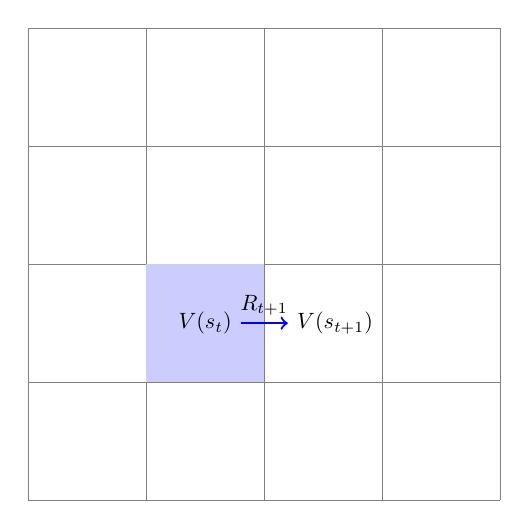
\begin{tikzpicture}[scale=1.5, every node/.style={scale=0.8}]
            \draw[step=1cm,gray,very thin] (0,0) grid (4,4);
            % Highlight current state
            \fill[blue!20] (1,1) rectangle (2,2);
            \node at (1.5,1.5) {$V(s_t)$};
            
            % Action taken from current state
            \draw[->, thick, blue] (1.8,1.5) -- (2.2,1.5);
            \node[above] at (2,1.5) {\(R_{t+1}\)};
            
            % Next state
            \node[] at (2.6,1.5) {$V(s_{t+1})$};

        \end{tikzpicture}
    \end{center}
\end{frame}

\begin{frame}{Bellman Equations development}
\begin{aligned}
V_{\pi}(s) &= \sum_{a \in \mathcal{A}} \pi(a \vert s) Q_{\pi}(s, a) \\
Q_{\pi}(s, a) &= R(s, a) + \gamma \sum_{s' \in \mathcal{S}} P_{ss'}^a V_{\pi} (s') \\
V_{\pi}(s) &= \sum_{a \in \mathcal{A}} \pi(a \vert s) \big( R(s, a) + \gamma \sum_{s' \in \mathcal{S}} P_{ss'}^a V_{\pi} (s') \big) \\
Q_{\pi}(s, a) &= R(s, a) + \gamma \sum_{s' \in \mathcal{S}} P_{ss'}^a \sum_{a' \in \mathcal{A}} \pi(a' \vert s') Q_{\pi} (s', a')
\end{aligned}
\end{frame}



\begin{frame}{The MDP Solution}
Dynamic Programming allows to resolve the MDP optimization problem ($\pi^* = \arg \max_{\pi} E_{\tau\sim \pi}[{G(\tau)}]$). It is an iterative process:
        \begin{itemize}
        \item{Policy initialization}
     \item{Policy evaluation}
     \item{Policy improvement}
            \end{itemize}
\end{frame}

\begin{frame}{Policy evaluation}
Policy Evaluation: compute the state-value $V_\pi$ for a given policy $\pi$:\\
We initialize $V_0$ arbitrarily. And we update it using:

\begin{aligned}
$V_{k+1}(s) &= \mathbb{E}_\pi [r + \gamma V_k(s_{t+1}) | S_t = s]\\
&= \sum_a \pi(a \vert s) \sum_{s'} P(s' \vert s, a) (R(s,a) + \gamma V_k(s'))$ (1)
\end{aligned}\\
$V_\pi(s)$ is a fix point for (1), so if $(V_k)_{k\in \mathbb{N}}$ converges, it converges to $V_\pi$.

\end{frame}

\begin{frame}{Policy Improvement}
Policy Improvement: generates a better policy $\pi' \geq \pi$ by acting greedily.
Compute $Q$ from $V$ ($\forall a,s$):
\begin{aligned}
Q_\pi(s, a) &= \mathbb{E} [R_{t+1} + \gamma V_\pi(S_{t+1}) \vert S_t=s, A_t=a]\\
&= \sum_{s'} P(s' \vert s, a) (R(s,a) + \gamma V_\pi(s'))
\end{aligned}

Update greedily: $\pi'(s) = \arg\max_{a \in \mathcal{A}} Q_\pi(s, a)$ ($\forall s$)
\end{frame}

\begin{frame}{Policy improvement: $\pi' (s) = \arg\max_{a \in A} Q_{\pi}(s, a)$}
    \begin{center}
        \begin{columns}
            \begin{column}{0.3\textwidth}
                \centering
                \( \pi: \)
        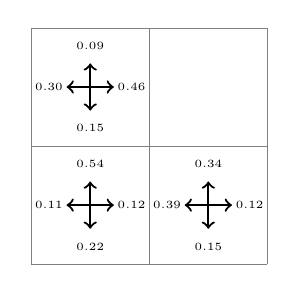
\begin{tikzpicture}[scale=1.5, every node/.style={scale=0.8}]
            \draw[step=1cm,gray,very thin] (0,0) grid (2,2);
            % Loop over each cell to draw arrows with random probabilities
            \foreach \x in {0,...,1}
                \foreach \y in {0,...,1}
                {
                                    % Generate four random numbers
                    \pgfmathsetmacro{\probup}{rnd}
                    \pgfmathsetmacro{\probdown}{rnd}
                    \pgfmathsetmacro{\probleft}{rnd}
                    \pgfmathsetmacro{\probright}{rnd}
                    % Calculate their sum
                    \pgfmathsetmacro{\sumprobs}{\probup + \probdown + \probleft + \probright}
                    % Normalize to sum up to 1
                    \pgfmathsetmacro{\probupnorm}{\probup / \sumprobs}
                    \pgfmathsetmacro{\probdownnorm}{\probdown / \sumprobs}
                    \pgfmathsetmacro{\probleftnorm}{\probleft / \sumprobs}
                    \pgfmathsetmacro{\probrightnorm}{\probright / \sumprobs}
                    % Draw arrows for each direction
                    % Up arrow
                    \ifthenelse{\NOT \x = 1 \OR \NOT \y = 1}{  
                    \draw[->, thick] (\x+0.5,\y+0.5) -- (\x+0.5,\y+0.7);
                    \node at (\x+0.5,\y+0.85) {\tiny \pgfmathprintnumber[fixed, fixed zerofill, precision=2]{\probupnorm}};
                    % Down arrow
                    \draw[->, thick] (\x+0.5,\y+0.5) -- (\x+0.5,\y+0.3);
                    \node at (\x+0.5,\y+0.15) {\tiny \pgfmathprintnumber[fixed, fixed zerofill, precision=2]{\probdownnorm}};
                    % Left arrow
                    \draw[->, thick] (\x+0.5,\y+0.5) -- (\x+0.3,\y+0.5);
                    \node at (\x+0.15,\y+0.5) {\tiny \pgfmathprintnumber[fixed, fixed zerofill, precision=2]{\probleftnorm}};
                    % Right arrow
                    \draw[->, thick] (\x+0.5,\y+0.5) -- (\x+0.7,\y+0.5);
                    \node at (\x+0.85,\y+0.5) {\tiny \pgfmathprintnumber[fixed, fixed zerofill, precision=2]{\probrightnorm}};}
                    }
        \end{tikzpicture}
            \end{column}
            
            \begin{column}{0.3\textwidth}
                \centering
                \( Q_{\pi}: \)
        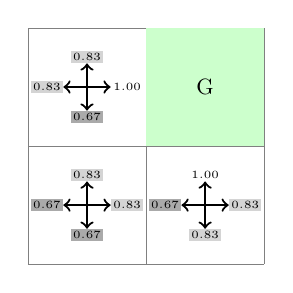
\begin{tikzpicture}[scale=1.5, every node/.style={scale=0.8}]
            \draw[step=1cm,gray,very thin] (0,0) grid (2,2);
            % Goal
            \fill[green!20] (1,1) rectangle (2,2);
            \node at (1.5,1.5) {G};

            % Loop over each cell to display Q-values for each action
            \foreach \x in {0,...,1}
                \foreach \y in {0,...,1}
                {
                
                    % Calculate Q-values based on Manhattan distance to the goal from the current cell
                    \pgfmathtruncatemacro{\UpY}{min(1,\y+1)}
                    \pgfmathtruncatemacro{\DownY}{max(0,\y-1)}
                    \pgfmathtruncatemacro{\LeftX}{max(0,\x-1)}
                    \pgfmathtruncatemacro{\RightX}{min(1,\x+1)}

                    % Calculate Manhattan distances for each action
                    \pgfmathsetmacro{\QupD}{abs(\x-1) + abs(\UpY-1)}
                    \pgfmathsetmacro{\QdownD}{abs(\x-1) + abs(\DownY-1)}
                    \pgfmathsetmacro{\QleftD}{abs(\LeftX-1) + abs(\y-1)}
                    \pgfmathsetmacro{\QrightD}{abs(\RightX-1) + abs(\y-1)}

                    \pgfmathsetmacro{\QupValue}{1 - (\QupD/6)}
                    \pgfmathsetmacro{\QdownValue}{1 - (\QdownD/6)}
                    \pgfmathsetmacro{\QleftValue}{1 - (\QleftD/6)}
                    \pgfmathsetmacro{\QrightValue}{1 - (\QrightD/6)}
                    
                    \definecolor{ColorUp}{rgb}{\QupValue, \QupValue, \QupValue}
                    \definecolor{ColorDown}{rgb}{\QdownValue, \QdownValue, \QdownValue}
                    \definecolor{ColorLeft}{rgb}{\QleftValue, \QleftValue, \QleftValue}
                    \definecolor{ColorRight}{rgb}{\QrightValue, \QrightValue, \QrightValue}
\ifthenelse{\NOT \x = 1 \OR \NOT \y = 1}{ 
                    % Draw arrows for each direction with corresponding Q-values
                    % Up arrow
                    \draw[->, thick] (\x+0.5,\y+0.5) -- (\x+0.5,\y+0.7);
                    \node[above, fill=ColorUp, inner sep=1pt] at (\x+0.5,\y+0.7) {\tiny \pgfmathprintnumber[fixed, fixed zerofill, precision=2]{\QupValue}};
                    % Down arrow
                    \draw[->, thick] (\x+0.5,\y+0.5) -- (\x+0.5,\y+0.3);
                    \node[below, fill=ColorDown, inner sep=1pt] at (\x+0.5,\y+0.3) {\tiny \pgfmathprintnumber[fixed, fixed zerofill, precision=2]{\QdownValue}};
                    % Left arrow
                    \draw[->, thick] (\x+0.5,\y+0.5) -- (\x+0.3,\y+0.5);
                    \node[left, fill=ColorLeft, inner sep=1pt] at (\x+0.3,\y+0.5) {\tiny \pgfmathprintnumber[fixed, fixed zerofill, precision=2]{\QleftValue}};
                    % Right arrow
                    \draw[->, thick] (\x+0.5,\y+0.5) -- (\x+0.7,\y+0.5);
                    \node[right, fill=ColorRight, inner sep=1pt] at (\x+0.7,\y+0.5) {\tiny \pgfmathprintnumber[fixed, fixed zerofill, precision=2]{\QrightValue}};}
                }
        \end{tikzpicture}
            \end{column}
            
            \begin{column}{0.05\textwidth}
                \centering
                \( \rightarrow \)
            \end{column}
            
            \begin{column}{0.3\textwidth}
                \centering
                \( \pi': \)
                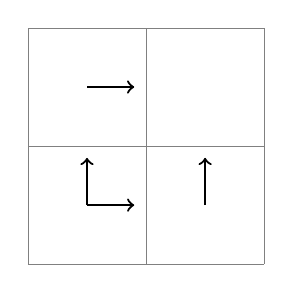
\begin{tikzpicture}[scale=1.5, every node/.style={scale=0.8}]
            \draw[step=1cm,gray,very thin] (0,0) grid (2,2);
            % Goal

            % Arrows pointing towards the goal "G"
            % Right arrows
            \foreach \y in {0,...,1}
                \foreach \x in {0,...,0}
                {
                    \draw[->, thick] (\x+0.5,\y+0.5) -- (\x+0.9,\y+0.5);
                }
            % Up arrows
            \foreach \x in {0,...,1}
                \foreach \y in {0,...,0}
                {
                    \draw[->, thick] (\x+0.5,\y+0.5) -- (\x+0.5,\y+0.9);
                }
                
            
        \end{tikzpicture}
            \end{column}
        \end{columns}
    \end{center}
\end{frame}


\begin{frame}{Dynamic Programming}
Policy Iteration: iterative procedure to improve the policy when combining policy evaluation and improvement.
\begin{equation}
    \pi_0 \xrightarrow[]{\text{evaluation}} V_{\pi_0} \xrightarrow[]{\text{improve}}
\pi_1 \xrightarrow[]{\text{evaluation}}\dots \xrightarrow[]{\text{improve}}
\pi_* \xrightarrow[]{\text{evaluation}} V_*
\end{equation}

\end{frame}
\begin{frame}{Bellman Equations Optimality}

Bellman equations for the optimal value functions


\begin{aligned}
V_*(s) &= \max_{a \in \mathcal{A}} Q_*(s,a)\\
Q_*(s, a) &= R(s, a) + \gamma \sum_{s' \in \mathcal{S}} P_{ss'}^a V_*(s') \\
V_*(s) &= \max_{a \in \mathcal{A}} \big( R(s, a) + \gamma \sum_{s' \in \mathcal{S}} P_{ss'}^a V_*(s') \big) \\
Q_*(s, a) &= R(s, a) + \gamma \sum_{s' \in \mathcal{S}} P_{ss'}^a \max_{a' \in \mathcal{A}} Q_*(s', a')
\end{aligned}
\end{frame}

\begin{frame}{Take home message}
Initialize $\pi(s), \forall s$
        \begin{enumerate}
        \item{Evaluate $V_\pi (s), \forall s$ (using $\mathbb{P}^a_{ss'}$)}
     \item{Compute $Q_\pi(s,a), \forall s,a$ (using $\mathbb{P}^a_{ss'}$)}
     \item{Update  $\pi'(s) = \max_a Q_\pi (s,a), \forall s$}
      \item{While $\pi'(s)$ \neq $\pi(s)$ do $\pi(s)$ = $\pi'(s)$ and iterate}
            \end{enumerate}
Result : $\pi = \arg \max_{\pi} E[G]$ 
\end{frame}
\begin{frame}[plain,c]
\begin{center}
\Huge Coding session

Dynamic Programming
\end{center}
\end{frame}
\end{document}

\end{document}
